\documentclass[idioma,boletin]{uah}

\tema{2}
\titulo{Modulaciones analógicas}{Analog modulations}
%
\begin{document}

\titulacion{Grados TIC}
\asignatura{Teoría de la Comunicación}{Communication Theory}
\departamento{Teoría de la Señal y Comunicaciones}
\curso{2021/2022} % Do not show year

\maketitle

\Problema{

		Una señal $x(t)$ periódica, de valor medio cero, ancho de banda $5 kHz$, amplitud máxima $4$ voltios y potencia media normalizada de $0.5$, modula en DBL a una portadora de $1 MHz$, obteniéndose una señal cuya potencia media es de $400 W$. Se pide:
		\begin{enumerate}
			\item Amplitud de la portadora.
			\item Potencia de la banda lateral inferior.
			\item Esquema del demodulador necesario para recuperar x(t), dando los valores más significativos del mismo.
		\end{enumerate}
		}
		{
		\begin{enumerate}
			\item $A_p = 10V$
			\item $P_{BLI} = 200W$
			\item Detector síncrono con $f_{OL}=1MHz$, $A_{OL}=\frac{2}{A_p}$ y $f_{pb} = 5kHz$.
		\end{enumerate}
		}
		{
	
		A zero-mean periodic signal $x(t)$, with bandwidth $5 kHz$, amplitude $4 V$ and normalized average power $0.5$, DSB modulates a $1MHz$ carrier. The result is a signal with average power $400 W$. Determine:
	
		\begin{enumerate}
			\item Carrier amplitude.
			\item Average power of the lower sideband.
			\item Outline of the detector needed to recover the signal x(t), and the value of its main parameters
		\end{enumerate}
		}
		{
		\begin{enumerate}
			\item $A_c = 10V$
			\item $P_{LSB} = 200W$
			\item Synchronous detector $f_{LO}=1MHz$, $A_{LO}=\frac{2}{A_c}$ and $f_{lp} = 5kHz$.
		\end{enumerate}
		}
		
			
\Problema{

	La señal $x(t) = cos(2\pi\cdot 10\cdot 10^3 t)+4\cdot cos(2\pi\cdot 15 \cdot10^3 t)+cos(2\pi \cdot 20\cdot10^3 t)$ modula en DBL a la portadora $p(t)=2\cdot cos(2\pi \cdot 10^5 t)$ y a continuación pasa a través de un filtro con respuesta $H(\omega)$ antes de llegar al detector, tal y como se puede ver en la figura.
	{\begin{figure*}[h!]\centering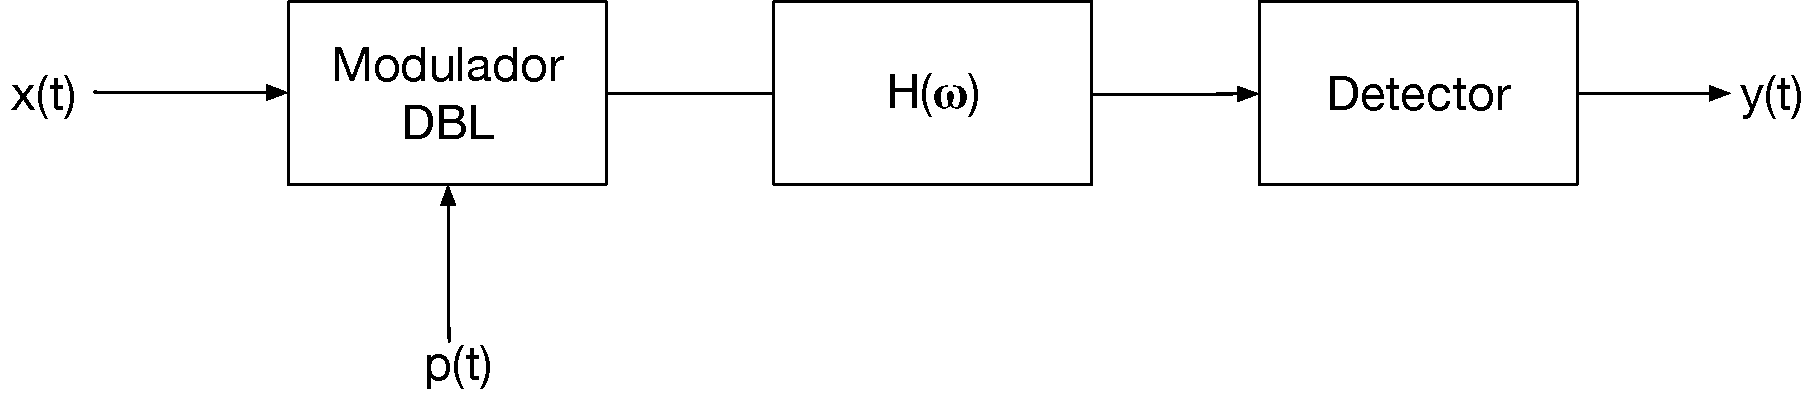
\includegraphics[width=10cm]{./Figuras/Problema2_2}\end{figure*}}


	donde
	\begin{displaymath}
		H(\omega)=\left \{ \begin{array}{ll}
			0 & |\omega|<200\pi krad/s  \\
			1 & |\omega|\geq200\pi krad/s
		\end{array}
		\right.
	\end{displaymath}

	\begin{enumerate}
		\item Hallar la señal que se obtendría a la salida si el detector empleado fuese un detector de envolvente con $K_D=1$ y supresión de continua.
		\item Determinar qué detector sería necesario para que la señal detectada coincidiese con la moduladora, especificando todos los parámetros necesarios.
	\end{enumerate} 
	}
	{
		\begin{enumerate}
			\item $y(t)=2\cdot cos(2\pi \cdot 5 \cdot 10^3t)$
			\item Detector síncrono con $f_{OL} = 2 \cdot cos(\omega_p \cdot t)$ y con filtro paso bajo con frecuencia de corte de al menos $20kHz$.
		\end{enumerate}
	}
	{

		The signal $x(t) = cos(2\pi\cdot 10\cdot 10^3 t)+4\cdot cos(2\pi\cdot 15 \cdot10^3 t)+cos(2\pi \cdot 20\cdot10^3 t)$ DSB modulates the carrier $p(t)=2\cdot cos(2\pi \cdot 10^5 t)$ and passes through a filter with frequency response $H(\omega)$ before reaching the detector, as it can be observed in the figure
		{\begin{figure*}[h!]\centering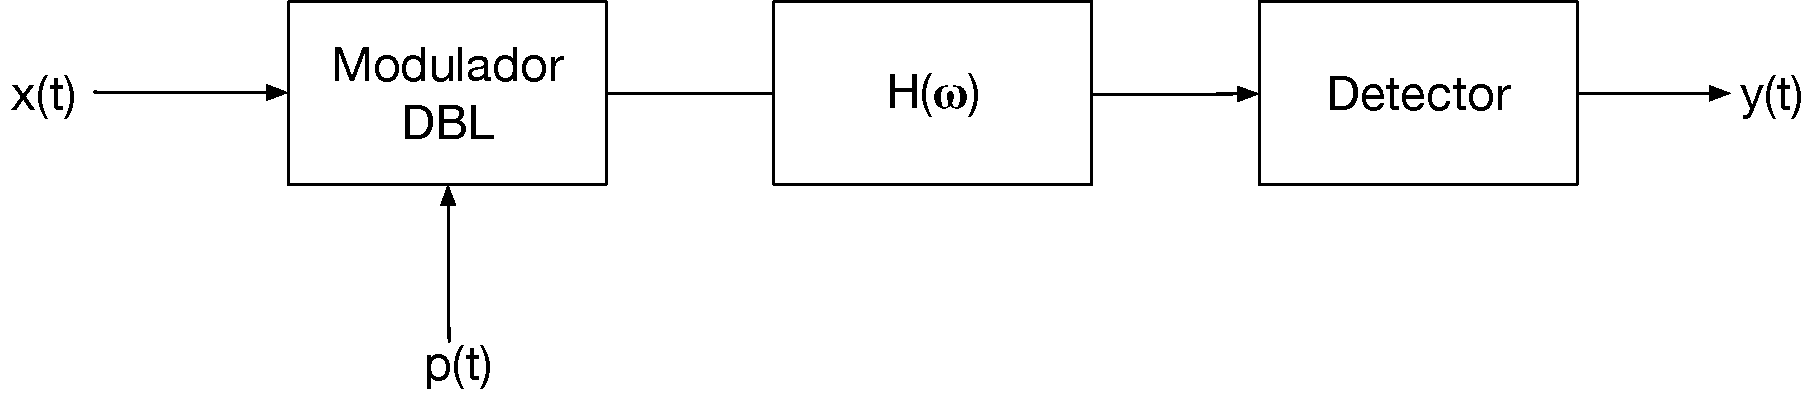
\includegraphics[width=10cm]{./Figuras/Problema2_2}\end{figure*}}
	
	
		with
		\begin{displaymath}
			H(\omega)=\left \{ \begin{array}{ll}
				0 & |\omega|<200\pi krad/s  \\
				1 & |\omega|\geq200\pi krad/s
			\end{array}
			\right.
		\end{displaymath}
	
		\begin{enumerate}
			\item Find the signal obtained at the output of the detector, when using an envelope detector of $K_D=1$ with DC suppression. 
			\item b)	Determine the detector needed to obtain a detected signal equal to the modulating signal. Please specify all necessary parameters.
		\end{enumerate} 
		}
		{
			\begin{enumerate}
				\item $y(t)=2\cdot cos(2\pi \cdot 5 \cdot 10^3t)$
				\item Synchronous detector with $f_{LO} = 2 \cdot cos(\omega_c \cdot t)$ 	and a low pass filter with cut-off frequency of at least $20kHz$.
			\end{enumerate}
		}
	
\Problema{

	Un transmisor tiene una potencia media nominal de $30 W$ y una potencia de pico máxima de $60 W$. Se pide calcular:
	
	\begin{enumerate}
		\item La potencia asociada a una banda lateral cuando la señal $x(t) = cos(\omega_m t)$ modula a la portadora $p(t)=A_p \cdot cos(\omega_p  t)$, así como el valor de $A_p$ en los casos siguientes:
			\begin{enumerate}
				\item Modulación AM al $80\%$.
				\item Modulación DBL
			\end{enumerate}
		\item En el primero de los casos del apartado anterior se observa que el canal presenta una atenuación no uniforme, tal como se aprecia en la figura. 
		{\begin{figure*}[h!]\centering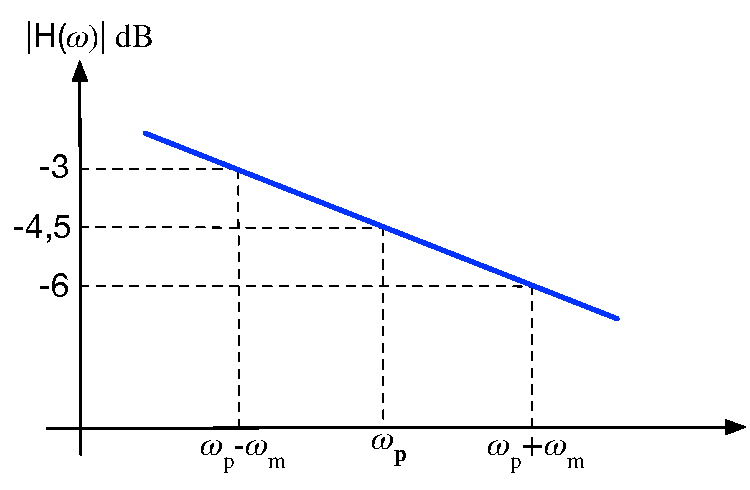
\includegraphics[width=6cm]{./Figuras/Problema2_3}\end{figure*}}
		Obtenga la señal detectada en los casos siguientes:
			\begin{enumerate}
				\item Detección de envolvente
				\item Detección síncrona
			\end{enumerate}
	\end{enumerate}
	
	\textsc{Nota:} En ambos casos se supondrá un bloque de supresión de continua.
}
{
\begin{enumerate}
	\item 
	\begin{enumerate}
		\item $A_p = 6.08V$, $P_{BL}=2.96W$
		\item $A_p = 10.95V$, $P_{BL}=15W$
	\end{enumerate}
	\item 
	\begin{enumerate}
		\item $y_D(t) = k_D\cdot \left [ A(t) - <A(t)>\right ]$, con:
			\begin{itemize}
				\item $A(t)=x_i(t) \cdot \left [ 1 + 0.5 \cdot \left ( \frac{x_q(t)}{x_i(t)} \right )^2 \right ]$
				\item $x_i(t)= 0.6 \cdot A_p + 0.48\cdot A_p \cdot cos(\omega_m t)$
				\item $x_q(t)=-0.08 \cdot A_p \cdot sen (\omega_m t)$
			\end{itemize}
		\item $y_D(t) = \frac{A_{OL}}{2} \cdot A_p \cdot 0.48 \cdot cos(\omega_m t)$
	\end{enumerate}
\end{enumerate}
}	
{

	A transmitter has an average nominal power of $30 W$ and a peak envelope power of $60 W$. Determine:

	\begin{enumerate}
		\item The power in a sideband when the signal $x(t) = cos(\omega_m t)$ modulates the carrier given by $p(t)=A_p \cdot cos(\omega_p t)$, and the value of $A_p$ in the following cases:
			\begin{enumerate}
				\item AM modulation when the modulation index is $80\%$.
				\item DSB modulation
			\end{enumerate}
		\item Considering the first case for a), and knowing that the channel presents a non-uniform attenuation as depicted in the figure:
		{\begin{figure*}[h!]\centering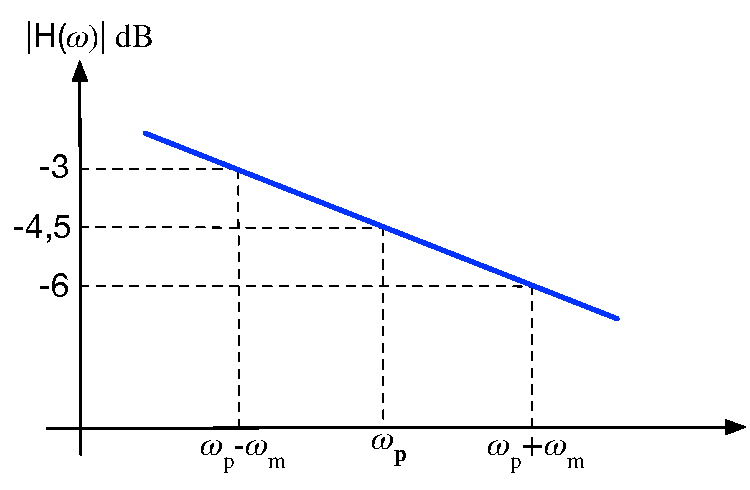
\includegraphics[width=6cm]{./Figuras/Problema2_3}\end{figure*}}
		Obtain the signal detected in the following cases:
			\begin{enumerate}
				\item Envelope detector
				\item Synchornous detector
			\end{enumerate}
	\end{enumerate}
	
	\textsc{Note:} Assume in both cases that a DC suppressor is present.
}
{
\begin{enumerate}
	\item 
	\begin{enumerate}
		\item $A_p = 6.08V$, $P_{BL}=2.96W$
		\item $A_p = 10.95V$, $P_{BL}=15W$
	\end{enumerate}
	\item 
	\begin{enumerate}
		\item $y_D(t) = k_D\cdot \left [ A(t) - <A(t)>\right ]$, con:
			\begin{itemize}
				\item $A(t)=x_i(t) \cdot \left [ 1 + 0.5 \cdot \left ( \frac{x_q(t)}{x_i(t)} \right )^2 \right ]$
				\item $x_i(t)= 0.6 \cdot A_p + 0.48\cdot A_p \cdot cos(\omega_m t)$
				\item $x_q(t)=-0.08 \cdot A_p \cdot sen (\omega_m t)$
			\end{itemize}
		\item $y_D(t) = \frac{A_{OL}}{2} \cdot A_p \cdot 0.48 \cdot cos(\omega_m t)$
	\end{enumerate}
\end{enumerate}
}

\newpage

\Problema {

	La señal $x(t)$, cuya frecuencia es $10 kHz$, modula a una portadora de $100 kHz$ y se observa en un osciloscopio una señal como la de la figura
	{\begin{figure*}[h!]\centering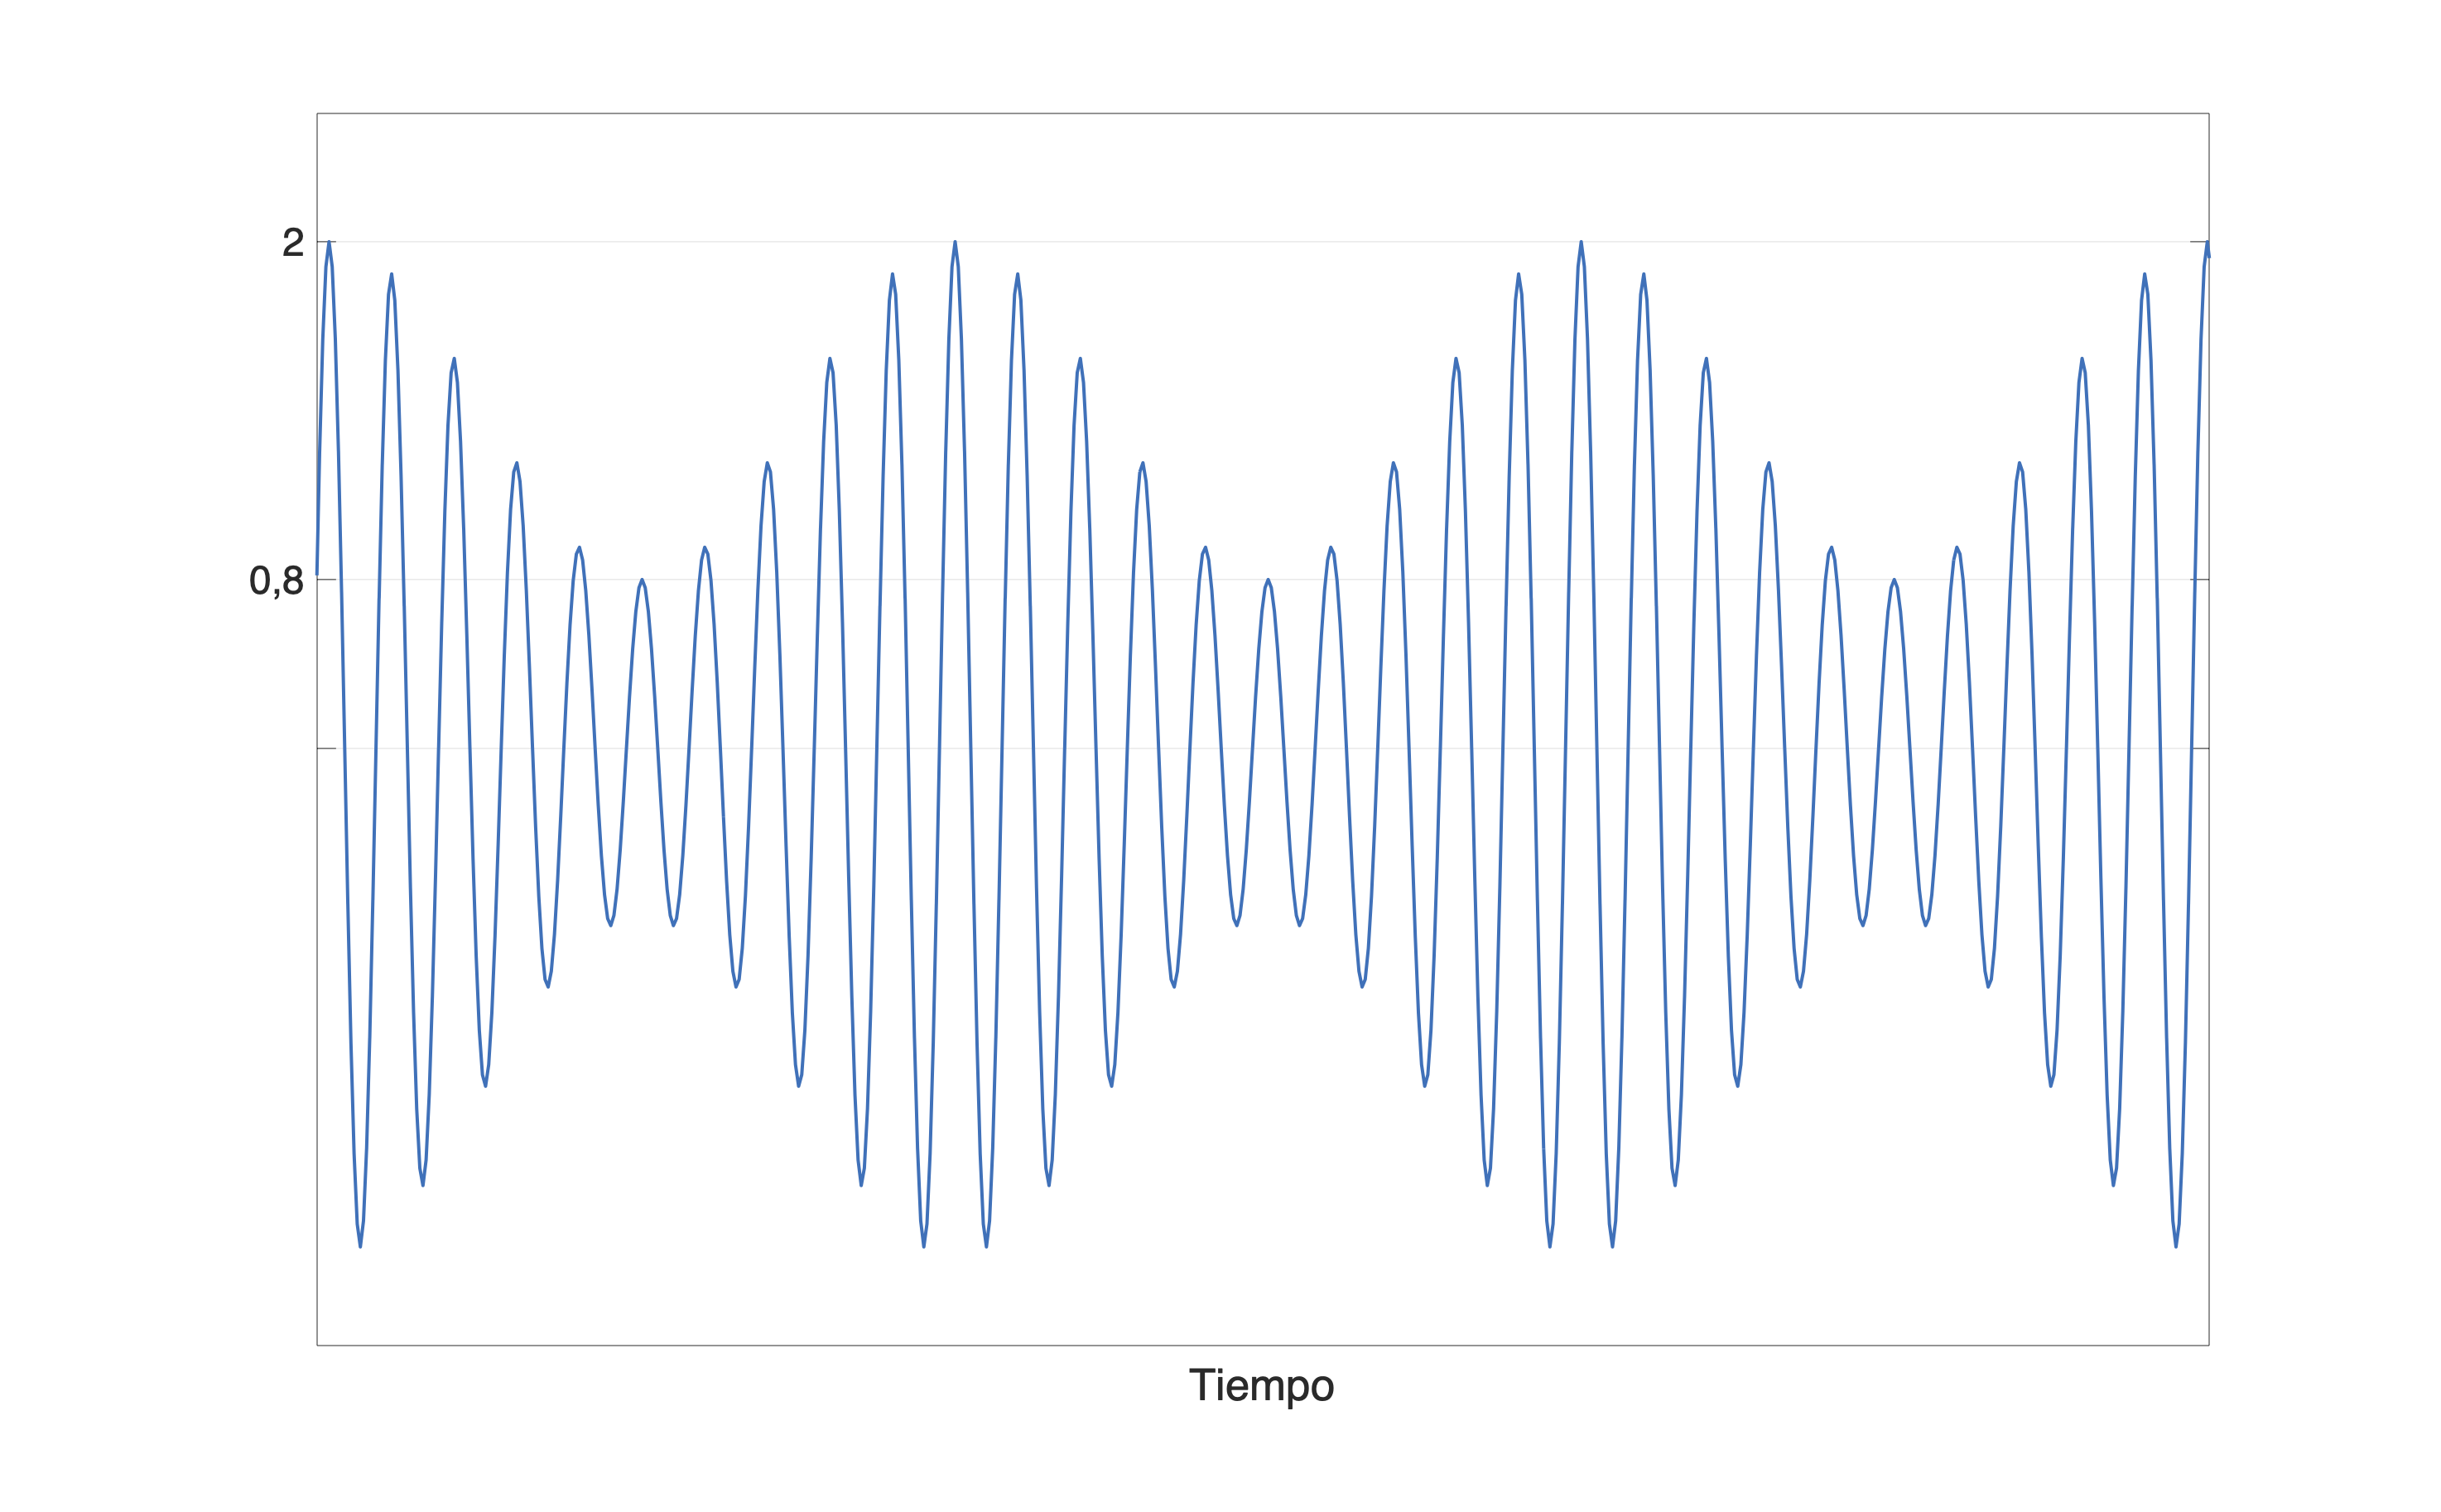
\includegraphics[width=12cm]{./Figuras/Problema2_4}\end{figure*}}
	Se pide:
	\begin{enumerate}
		\item Indicar el tipo de modulación utilizado.
		\item Obtener el índice de modulación.
		\item Obtener la potencia de la portadora y de la moduladora normalizada.
		\item Obtener la señal recuperada si se utiliza un detector síncrono, sintonizado a $100 kHz$ y de amplitud $1V$.
		\item Obtener la señal recuperada si se utiliza un detector de envolvente.
	\end{enumerate}	
	
	\textsc{Nota}: Puede suponerse que $K_D =1$.
}
{
\begin{enumerate}
	\item AM
	\item $m \approx 0.43$
	\item $P_p = 0.98 W$, $S_{xn} = 0.5$
	\item $y_D(t)=0.3 \cdot cos(2\pi \cdot 10^4t)$
	\item $y_D(t)=0.6 \cdot cos (2\pi \cdot 10^4t)$
\end{enumerate}
}
{

	A $10 kHz$ signal $x(t)$ modulates a $100 kHz$ carrier and the result, as observed using an oscilloscope, is presented in the figure. 
	{\begin{figure*}[h!]\centering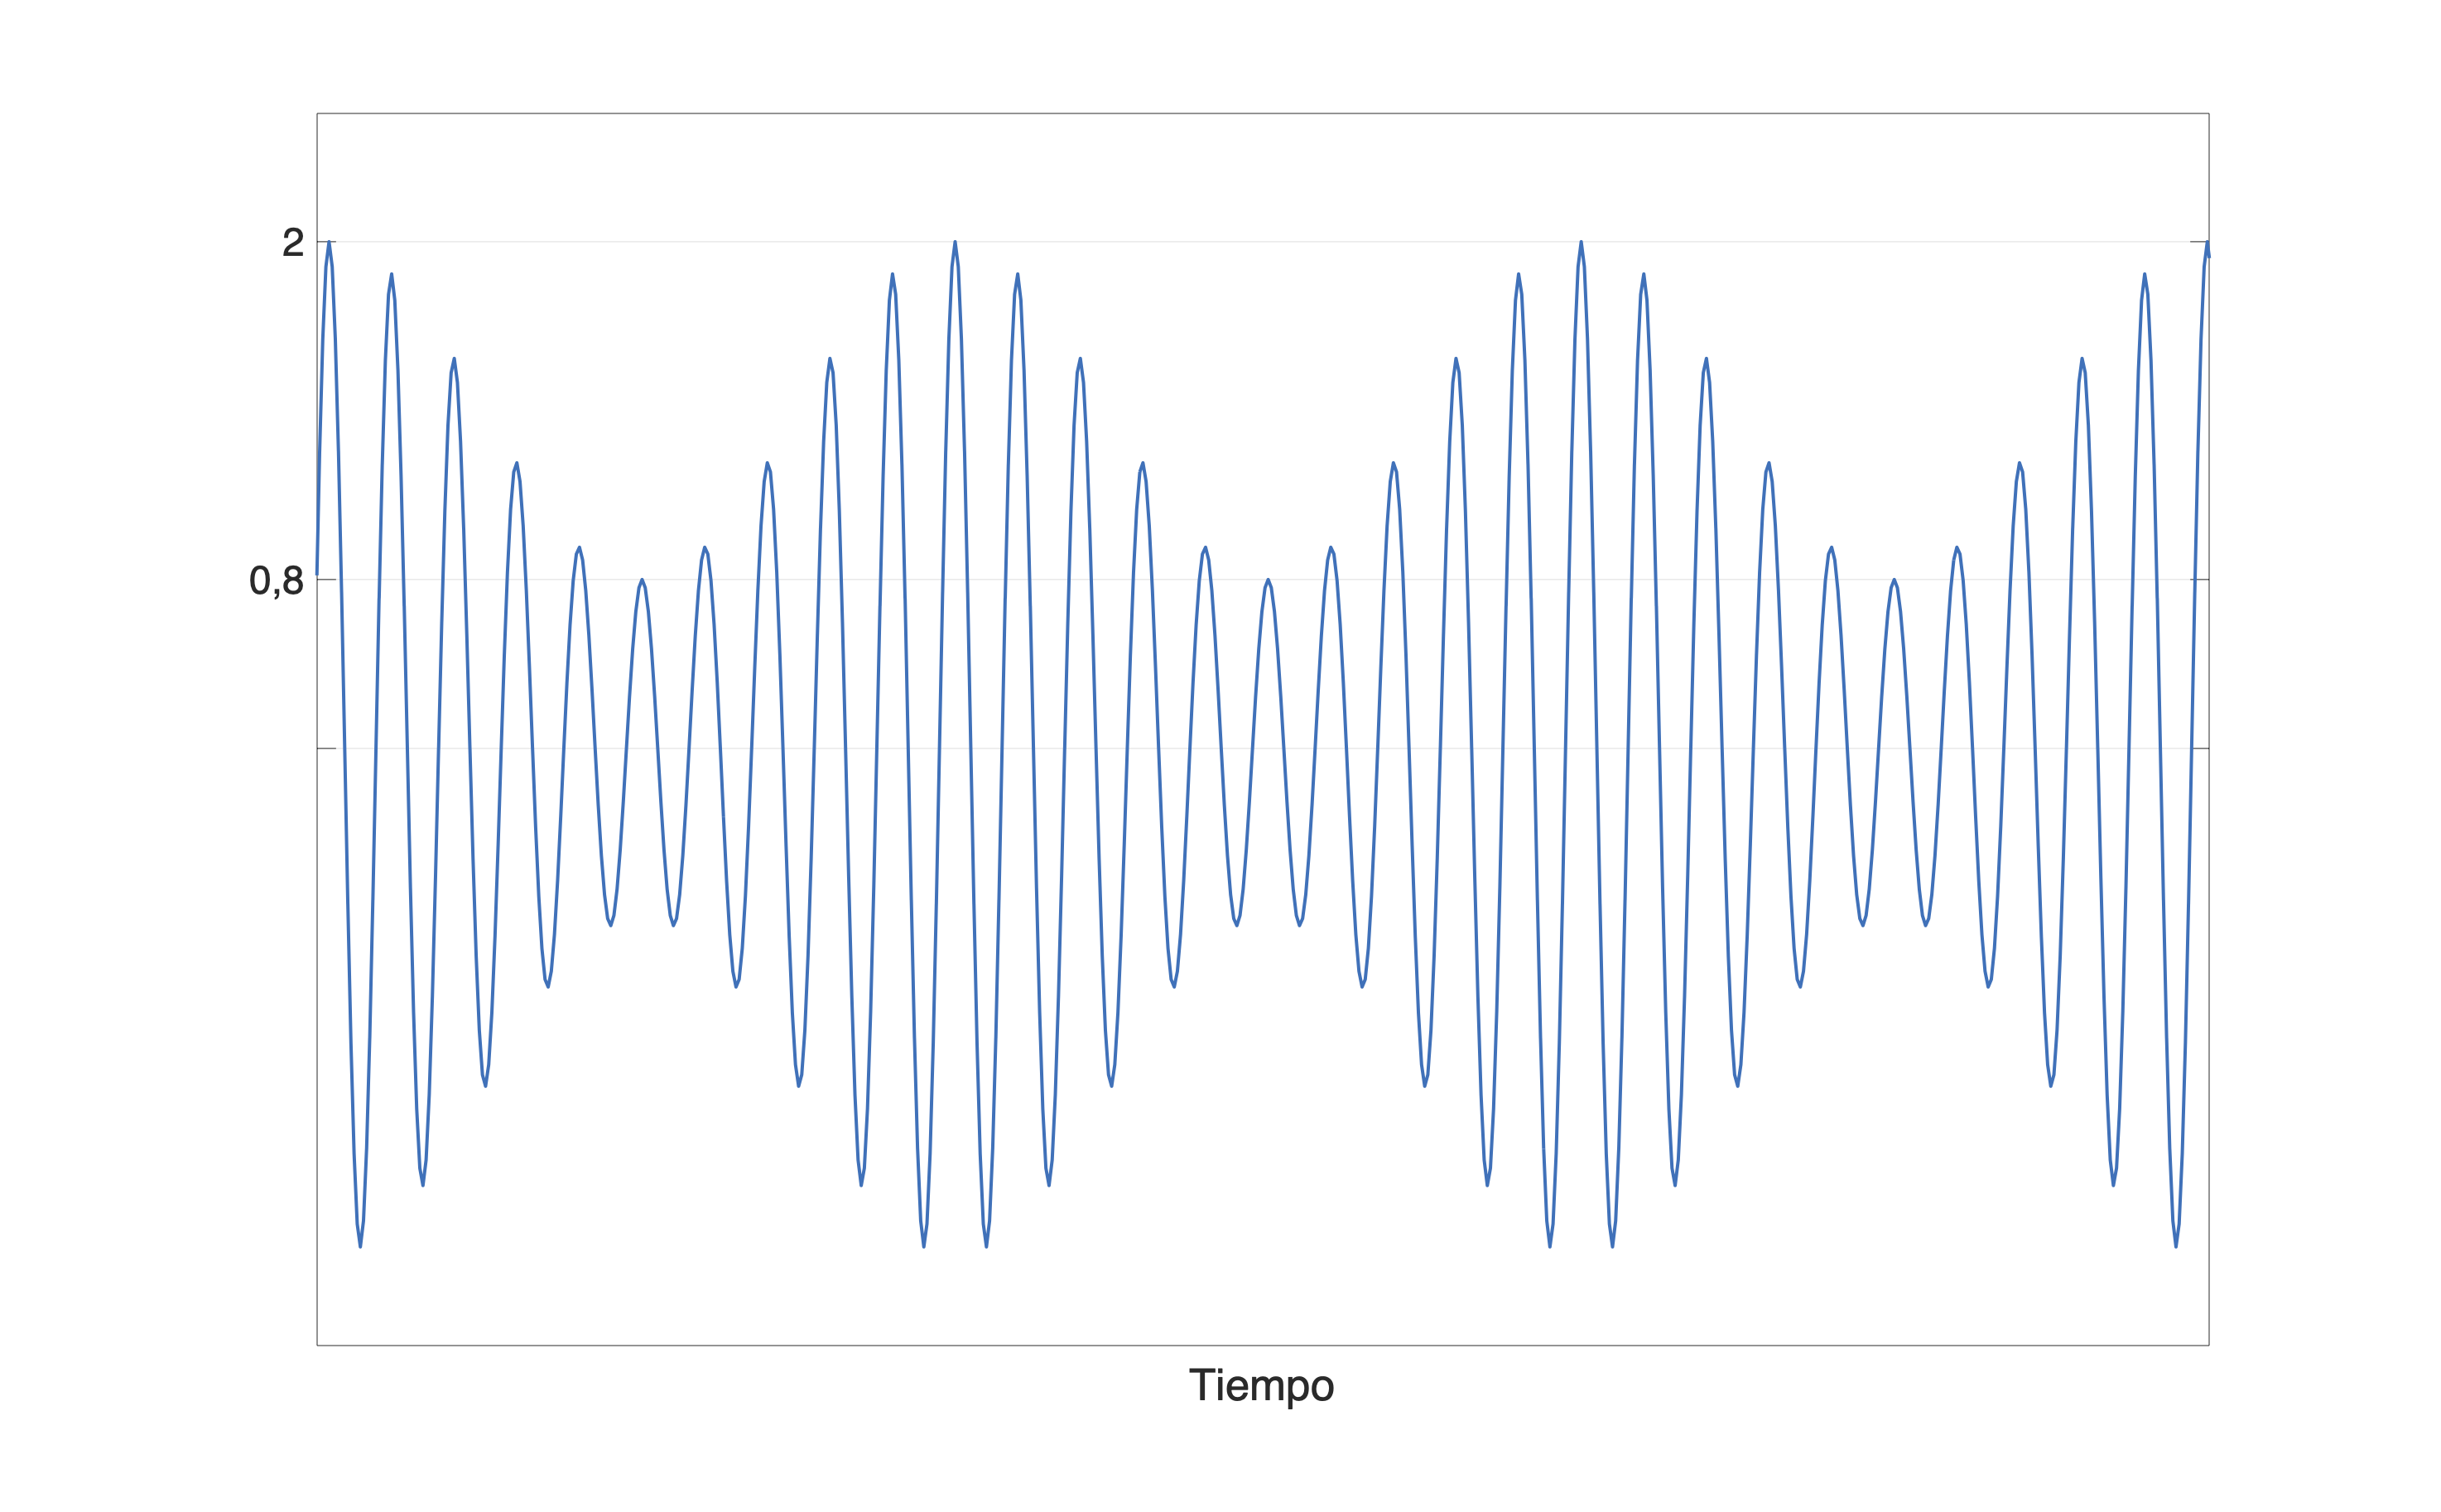
\includegraphics[width=12cm]{./Figuras/Problema2_4}\end{figure*}}
	Determine:
	\begin{enumerate}
		\item Modulation used.
		\item Modulation index.
		\item Carrier's power and Modulating signal's normalized power. Recovered signal when using a synchronous detector tuned to $100 kHz$ and with an amplitude of $1V$.
		\item Recovered signal when using an envelope detector.
	\end{enumerate}	
	
	\textsc{Note}: It can be assumed that $K_D=1$.
}
{
\begin{enumerate}
	\item AM
	\item $m \approx 0.43$
	\item $P_p = 0.98 W$, $S_{xn} = 0.5$
	\item $y_D(t)=0.3 \cdot cos(2\pi \cdot 10^4t)$
	\item $y_D(t)=0.6 \cdot cos (2\pi \cdot 10^4t)$
\end{enumerate}
}

\newpage

\Problema{

	Si $x_{FM}(t)$ es la señal que resulta al modular en FM una portadora $p(t)=A_p \cdot cos(\omega_p t)$ por una señal $x(t)$. ¿Cuál sería la condición que permitiría recuperar la señal $x(t)$ mediante el circuito de la figura?
	{\begin{figure*}[h!]\centering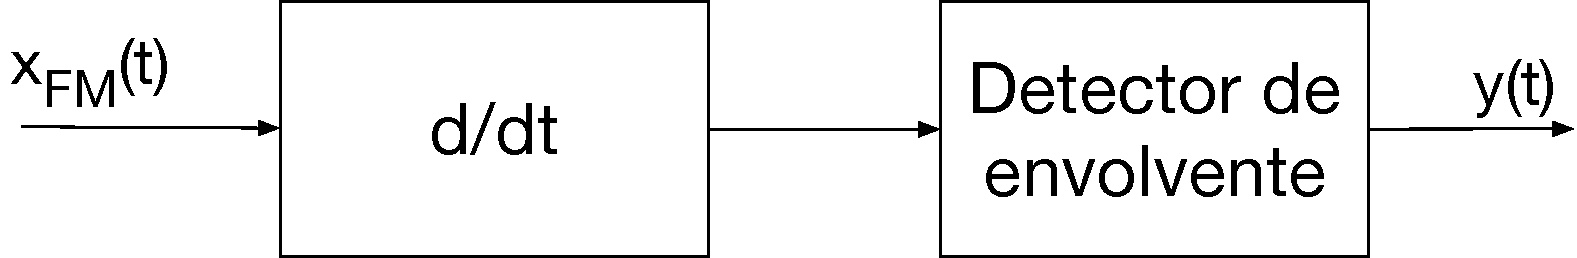
\includegraphics[width=8cm]{./Figuras/Problema2_5}\end{figure*}}
}
{
$\omega_p - \omega_\Delta \cdot |x(t)|_{max} > 0$

}
{

	Considering that $x_{FM}(t)$ is the signal obtained when FM modulating a signal $x(t)$ with the carrier $p(t)=A_p \cdot cos(\omega_p t)$. Determine the condition needed to recover the signal $x(t)$ if the system outlined in the figure is used.
	
	{\begin{figure*}[h!]\centering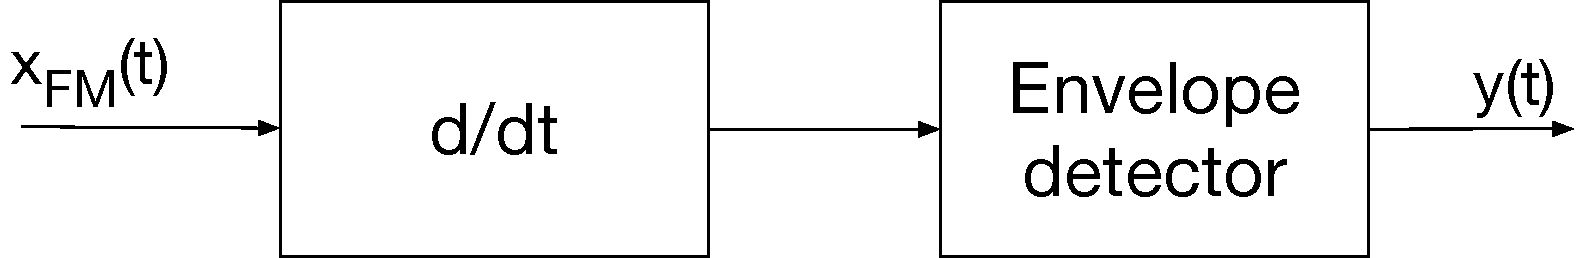
\includegraphics[width=8cm]{./Figuras/Problem2_5}\end{figure*}}
}
{
$\omega_p - \omega_\Delta \cdot |x(t)|_{max} > 0$

}


\Problema {

	El esquema de la figura representa un modulador de FM seguido de un convertidor de frecuencia y un filtro paso banda para adaptar la señal modulada a una banda de frecuencias conveniente para la transmisión. Para ajustar los parámetros del sistema se utiliza un tono de prueba $x(t)$. A partir de los valores recogidos en el apartado de datos, se pide calcular:
	
	\begin{enumerate}
		\item El índice de modulación $D$ y el ancho de banda de la onda modulada.
		\item El valor del ancho de banda, $B$, y la pulsación central del filtro, $\omega_0$, sabiendo que la banda de frecuencias que se nos ha asignado para la transmisión está situada por encima de $\omega_1$.
		\item La potencia de la señal $y(t)$ sabiendo que el filtro atenúa la señal un $10\%$. Dejar el resultado en función de $A_p$.
	\end{enumerate}
	{\begin{figure*}[h!]\centering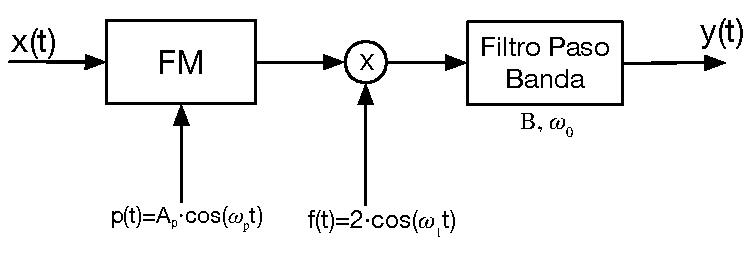
\includegraphics[width=12cm]{./Figuras/Problema2_6}\end{figure*}}
	\textsc{Datos:}
	\begin{itemize}
		\item $x(t) = cos(\omega_m t) \,\, [V]$
		\item $\omega_m = 2\pi \cdot 4 krad/s$
		\item $\omega_p = 2\pi \cdot 400 krad/s$
		\item $\omega_1 = 2\pi \cdot 2 Mrad/s$
		\item $\omega_d = 2\pi \cdot 16 krad/s\cdot V$
	\end{itemize}
}
{
\begin{enumerate}
	\item $D=4$, $B_T = 2\pi \cdot 48 krad/s$
	\item $\omega_0 = \omega_1 + \omega_p$, $B \geq B_T$
	\item $P_y = 0.81 \cdot \frac{A_p^2}{2}$
\end{enumerate}
}
{

	The outline presented in the figure shows a FM modulator followed by a frequency converter and a band-pass filter (used to adapt the modulated signal to a suitable transmission frequency band). In order to set the system's parameters, a test tone $x(t)$ is used. Determine:
	
	\begin{enumerate}
		\item Modulation index $D$, and modulated signal's bandwidth.
		\item Value of the filter's bandwidth, $B$, and the filter's central frequency, $\omega_0$, considering that a frequency band that is above $\omega_1$ has been assigned for our transmission.
		\item Average power of the output $y(t)$ as a function of $A_p$ considering that the filter attenuates the signal a $10\%$.
	\end{enumerate}

	{\begin{figure*}[h!]\centering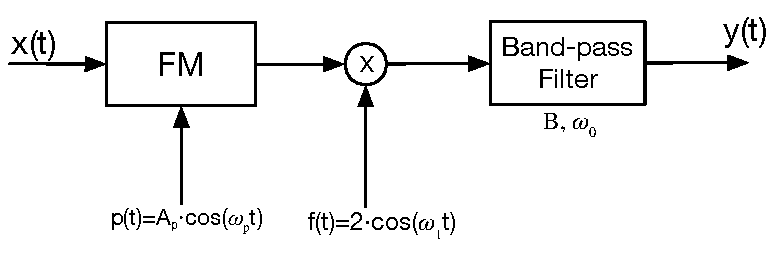
\includegraphics[width=10cm]{./Figuras/Problema2_6_en}\end{figure*}}
	
	\textsc{Data:}
	\begin{itemize}
		\item $x(t) = cos(\omega_m t) \,\, [V]$
		\item $\omega_m = 2\pi \cdot 4 krad/s$
		\item $\omega_p = 2\pi \cdot 400 krad/s$
		\item $\omega_1 = 2\pi \cdot 2 Mrad/s$
		\item $\omega_d = 2\pi \cdot 16 krad/s\cdot V$
	\end{itemize}
}
{
\begin{enumerate}
	\item $D=4$, $B_T = 2\pi \cdot 48 krad/s$
	\item $\omega_0 = \omega_1 + \omega_p$, $B \geq B_T$
	\item $P_y = 0.81 \cdot \frac{A_p^2}{2}$
\end{enumerate}
}

\Problema{

	La señal $x(t) = cos(\omega_1 t) + cos(\omega_2 t)$ modula en FM a la portadora $p(t) = A_p\cdot cos(\omega_p t)$. La señal modulada es pasada por un filtro paso alto con frecuencia de corte $2\pi\cdot 350 krad/s$, y la señal resultante se pasa por un detector síncrono en el que el oscilador local está ajustado a la frecuencia de la portadora considerada, estando su expresión dada por $p_{OL} (t)$ (ver Datos y Figura).  
	
	{\begin{figure*}[h!]\centering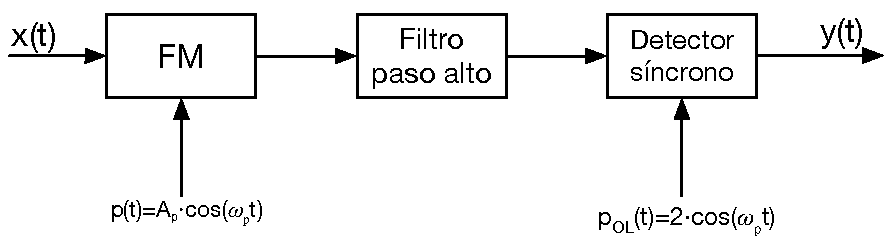
\includegraphics[width=10cm]{./Figuras/Problema2_7}\end{figure*}}
	
	Se pide calcular la señal resultante del sistema, $y(t)$, en función de $A_p$.
	
	\textsc{Datos:}
	\begin{itemize}
		\item $\omega_1 = 2\pi \cdot 64 krad/s$
		\item $\omega_2 = 2\pi \cdot 128 krad/s$
		\item $\omega_d = 2\pi \cdot 2 krad/s \cdot V$
		\item $\omega_p = 2\pi \cdot 400 krad/s$
		\item $p_{OL}(t) = 2 \cdot cos(\omega_p t)$
	\end{itemize}
}
{
$y(t)=A_p \cdot \left [ 1 + \left ( \frac{\omega_d}{2 \omega_1} \right ) cos(\omega_1 t) + \left ( \frac{\omega_d}{2\omega_2} \right ) cos(\omega_2 t) \right]$
\ \\
 
}
{

	The signal $x(t) = cos(\omega_1 t) + cos(\omega_2 t)$ FM modulates the carrier $p(t) = A_p\cdot cos(\omega_p t)$. The modulated signal goes through a high pass filter with cutoff frequency $2\pi\cdot 350 krad/s$, whose output signal is fed to a synchronous detector where the local oscillator is adjusted to the carrier frequency, following the expression given by $p_{OL} (t)$ (see Data and Figure). 
	
	{\begin{figure*}[h!]\centering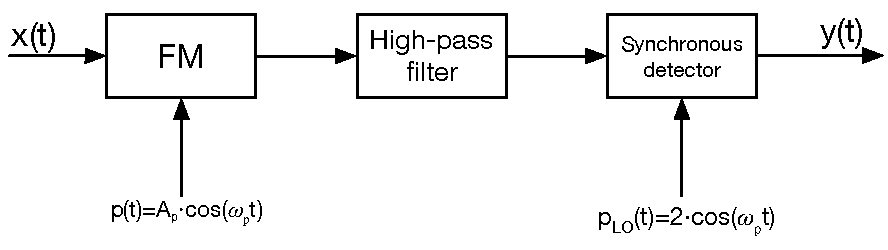
\includegraphics[width=10cm]{./Figuras/Problem2_7}\end{figure*}}
	
	Calculate the output signal $y(t)$ as a function of $A_p$.
	
	\textsc{Datos:}
	\begin{itemize}
		\item $\omega_1 = 2\pi \cdot 64 krad/s$
		\item $\omega_2 = 2\pi \cdot 128 krad/s$
		\item $\omega_d = 2\pi \cdot 2 krad/s \cdot V$
		\item $\omega_p = 2\pi \cdot 400 krad/s$
		\item $p_{OL}(t) = 2 \cdot cos(\omega_p t)$
	\end{itemize}
}
{
$y(t)=A_p \cdot \left [ 1 + \left ( \frac{\omega_d}{2 \omega_1} \right ) cos(\omega_1 t) + \left ( \frac{\omega_d}{2\omega_2} \right ) cos(\omega_2 t) \right]$
\ \\
 
}

\Problema{

Un tono $x(t)$, de frecuencia $1 kHz$ y $1 V$ de amplitud, modula a una portadora $p(t)$ de $1 MHz$, generándose una señal $y(t)$ como la que se muestra en la siguiente figura, cuya envolvente varía entre $1 V$ y $7 V$.

{\begin{figure*}[h!]\centering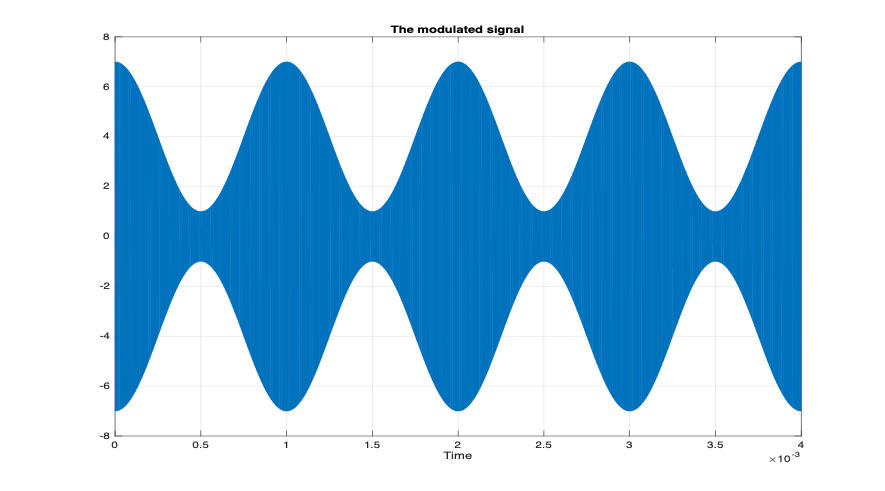
\includegraphics[width=10cm]{./Figuras/Imagen2_7}\end{figure*}}

\begin{enumerate}
	\item 	Indique el tipo de modulación utilizado y determine el valor del índice de modulación y de la amplitud de la señal portadora (indicando sus unidades).
	\item Dibuje el espectro de la señal modulada, y(t), indicando los valores de amplitud y frecuencias.

\end{enumerate}
Ahora se desea modular la portadora $p(t)$ en FM con el tono $x(t)$. El modulador FM tiene una desviación de frecuencia de $15 kHz/V$.

\begin{enumerate}\setcounter{enumi}{2}
	\item Dibuje, aproximadamente, la señal en el dominio del tiempo que se obtendría cuando el tono de partida $x(t)$ module en FM a $p(t)$. Indique los valores entre los que varía la envolvente. 

	\item ¿Es posible obtener la señal moduladora empleando el siguiente esquema?
		
	{\begin{figure*}[h!]\centering
	\begin{subfigure}{}
	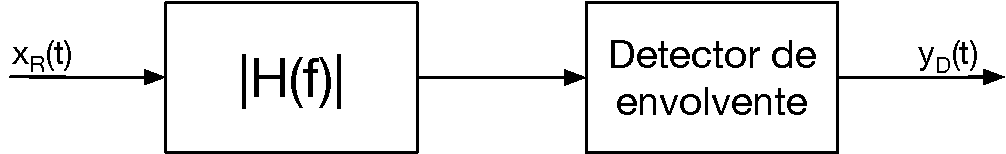
\includegraphics[width=6cm]{./Figuras/Problema2_8a}
	\end{subfigure}
	\begin{subfigure}{}
	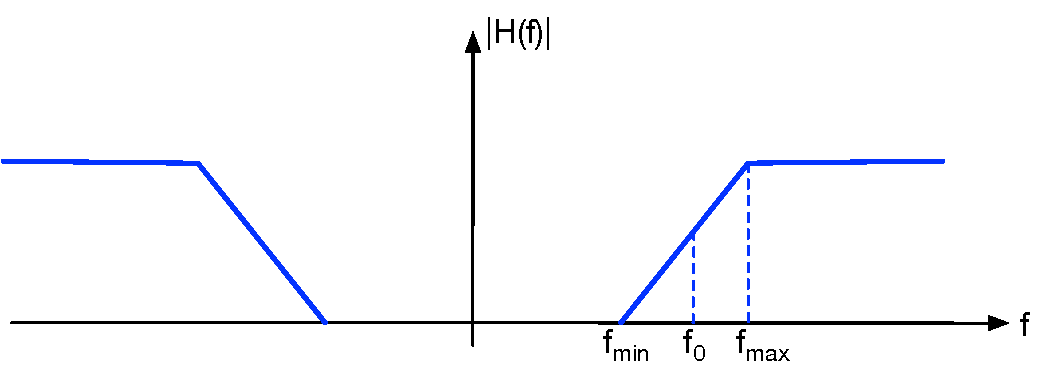
\includegraphics[width=6cm]{./Figuras/Problema2_8b}
	\end{subfigure}
	\end{figure*}}
\end{enumerate}

}
{
\begin{enumerate}
	\item Es una modulación AM con $m=0.75$ y $A_p = 4V$.
	\item $Y(\omega) = 4\pi \left [ \delta (\omega-\omega_p) + \delta(\omega+\omega_p)\right ] + \\
		+ \left ( \frac{3\pi}{2} \right ) \cdot \left [ \delta(\omega-\omega_p-\omega_m) + \delta(\omega-\omega_p+\omega_m) + \delta(\omega+\omega_p-\omega_m) + \delta(\omega+\omega_p+\omega_m)\right ]$
	\item $[-A_p, A_p]$
	\item Sí que es posible.
\end{enumerate}
}
{

A given $1 kHz$ frequency tone $x(t)$, with a $1 V$ amplitude, DSB-AM modulates a $1 MHz$ carrier $c(t)$. The following figure shows the modulated signal $y(t)$ characterized by a maximum value of $7 V$, and a minimum value of $1 V$.

{\begin{figure*}[h!]\centering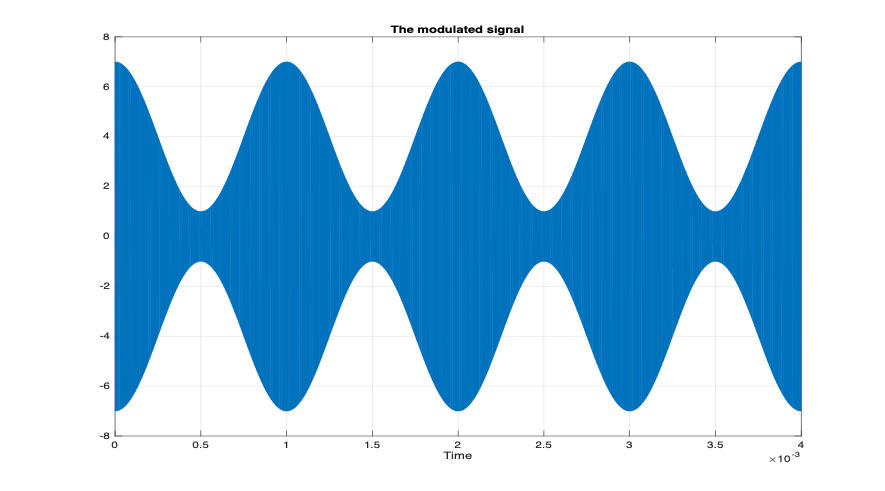
\includegraphics[width=10cm]{./Figuras/Imagen2_7}\end{figure*}}

\begin{enumerate}
	\item State the type of modulation and determine the modulation index as well as the carrier's amplitude (with its units).
	\item Plot the modulated signal, $y(t)$, spectrum showing in the plot the specific amplitude and frequency values.
\end{enumerate}

At this point, we want to modulate the carrier $c(t)$ in frequency (FM) using the tone $x(t)$. The FM modulator has a frequency deviation of $15 kHz$.

\begin{enumerate}\setcounter{enumi}{2}
	\item Plot, roughly, the time-domain signal obtained when the tone x(t) modulates in frequency (FM) the same carrier $c(t)$. Please provide the envelope's amplitude range value.

	\item Is it possible to obtain the modulated signal using the following scheme?
	
	{\begin{figure*}[h!]\centering
	\begin{subfigure}{}
	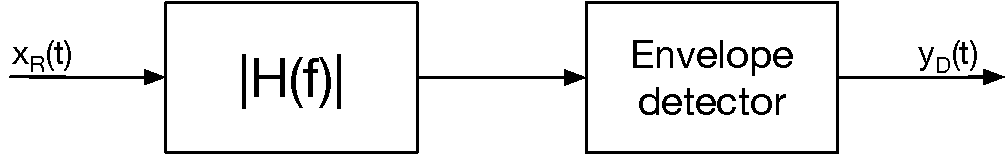
\includegraphics[width=6cm]{./Figuras/Problem2_8a}
	\end{subfigure}
	\begin{subfigure}{}
	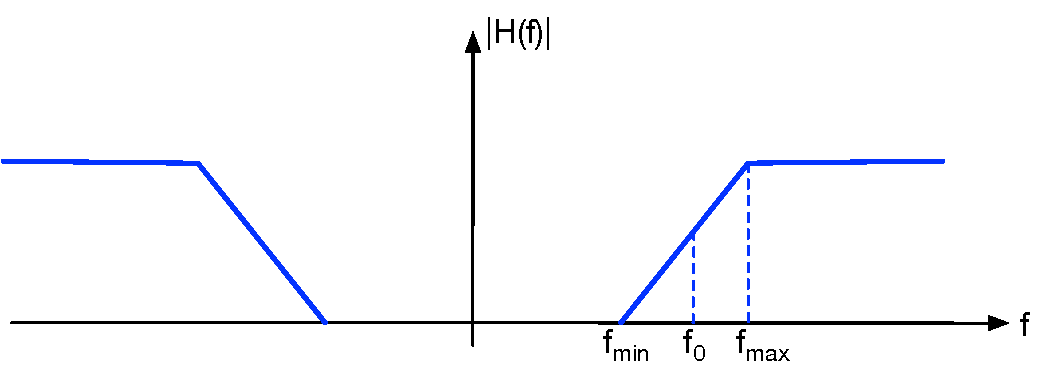
\includegraphics[width=6cm]{./Figuras/Problema2_8b}
	\end{subfigure}
	\end{figure*}}
\end{enumerate}

}
{
\begin{enumerate}
	\item It is an AM modulation with $m=0.75$ y $A_p = 4V$.
	\item $Y(\omega) = 4\pi \left [ \delta (\omega-\omega_p) + \delta(\omega+\omega_p)\right ] + \\
		+ \left ( \frac{3\pi}{2} \right ) \cdot \left [ \delta(\omega-\omega_p-\omega_m) + \delta(\omega-\omega_p+\omega_m) + \delta(\omega+\omega_p-\omega_m) + \delta(\omega+\omega_p+\omega_m)\right ]$
	\item $[-A_p, A_p]$
	\item Yes, it is possible.
\end{enumerate}
}


\end{document}



	
